\documentclass[a4paper]{article}
\usepackage[utf8]{inputenc}
\usepackage[T1]{fontenc}
\usepackage[pdftex]{graphicx}
\usepackage{fancyhdr}
\usepackage{lscape}
\usepackage{color}
\usepackage{qtree}
\usepackage[english]{babel}
\usepackage{graphicx}
\usepackage[colorinlistoftodos]{todonotes}
\usepackage{listings}
\usepackage{color}
\usepackage{float}
\usepackage{changepage}
\usepackage[margin=1in]{geometry}
\definecolor{codegreen}{rgb}{0,0.6,0}
\definecolor{codegray}{rgb}{0.5,0.5,0.5}
\definecolor{codepurple}{rgb}{0.58,0,0.82}
\definecolor{backcolour}{rgb}{0.95,0.95,0.92}
\usepackage[final]{pdfpages} 
\usepackage[parfill]{parskip}

 
 \lstdefinestyle{mystyle}{
 	backgroundcolor=\color{backcolour},   
 	commentstyle=\color{codegreen},
 	keywordstyle=\color{magenta},
 	numberstyle=\tiny\color{codegray},
 	stringstyle=\color{codepurple},
 	basicstyle=\footnotesize,
 	breakatwhitespace=false,         
 	breaklines=true,                 
 	captionpos=b,                    
 	keepspaces=true,                 
 	numbers=left,                    
 	numbersep=5pt,                  
 	showspaces=false,                
 	showstringspaces=false,
 	showtabs=false,                  
 	tabsize=2
 }
 
\lstset{
	style=mystyle,
	inputencoding=utf8,
	extendedchars=true,
	literate={á}{{\'a}}1 {ã}{{\~a}}1 {é}{{\'e}}1,
	escapechar=\&
}
\title{Algorithmique et structures de données : Mission 5}
\date{28 novembre 2014}
\author{Groupe 1.2: Ivan Ahad - Jérôme Bertaux - Rodolphe Cambier \\ 
	Baptiste Degryse - Wojciech Grynczel - Charles Jaquet}

\begin{document}
\maketitle


Rapport écrit par Rodolphe Cambier, Ivan Ahad
\section*{Introduction}
La mission pour cette semaine était de créer un programme permettant de compresser et de décompresser des textes à l'aide du codage de Huffman. 

\section*{Questions par rapport au programme}

\subsubsection*{Question 7}

IntputBytestream et OutputBytesream permettent respectivement la lecture et l’écriture en bit à bit.
La méthode close est par exemple appelée dans une situation telle que notre texte à compresser contient seulement 11 fois le caractère “a”. Ainsi, la compression se fera sur 11 bits. La méthode “close” va donc combler les 5 bits manquant pour atteindre le multiple de 8. La conséquence sur notre programme est que l’on rajoute un caractère “EOF” (end of file) pour ne pas tenir compte des 0 à la fin du fichier, ainsi la lecture s’arrêtera lorsque l’on tombe sur ce EOF. 


\subsubsection*{Question 8 - Diagramme UML}

La classe commune entre le programme de compression et de décompression est OutputByteStream. 
\\
La classe Entry et Node implémentent l'interface comparable. 

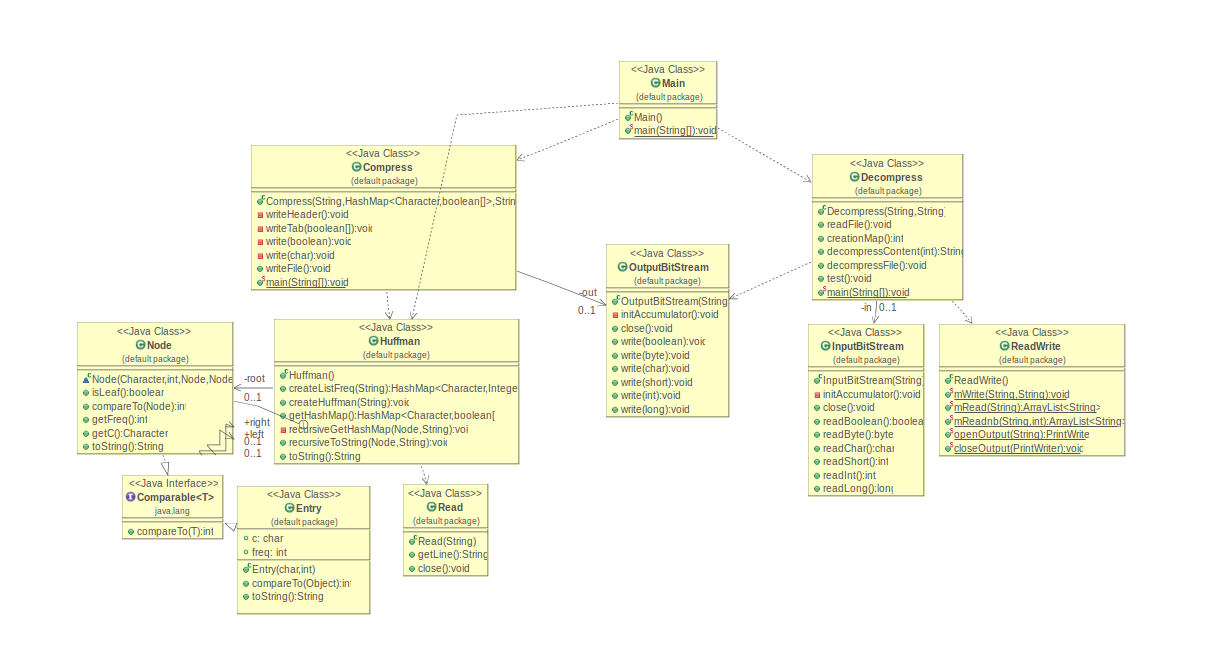
\includegraphics[scale=0.45]{UML.png}
\subsubsection*{Question 9}
Le taux de compression dépend à la fois de la taille du fichier et du nombre de caractères différents utilisés. Dans un cas extême, si de nombreux caractères différents sont utilisés dans un texte très court, le fichier compressé sera plus lourd que le fichier d'origine. C'est dû au fait qu'on ajoute le mapping des lettres à leur représentation en bits en début du fichier compressé.\\

Par exemple, tenter de compresser un fichier contenant seulement les caractères "abdefghijklmnopqrstuvwxyz", le fichier original est de 26 bytes, et le fichier compressé est de 110 bytes. 
\\
Le programme ne devient efficace qu'à partir d'un certain nombre de caractères. 
\\

%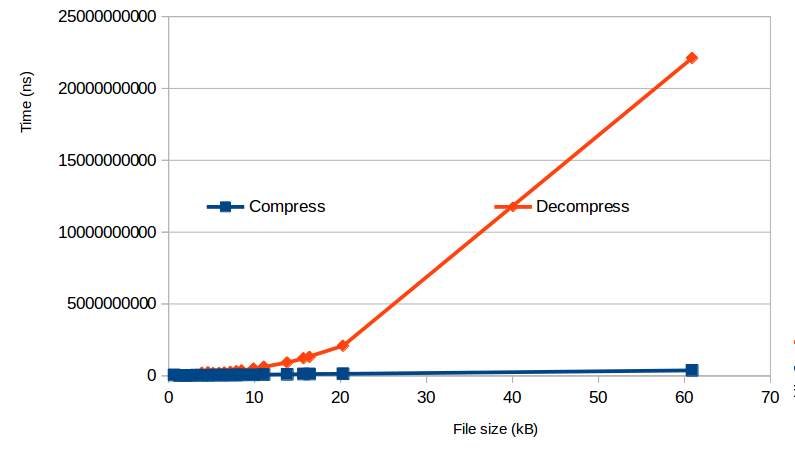
\includegraphics[scale=0.39]{graph.png}
\begin{figure}[b]
   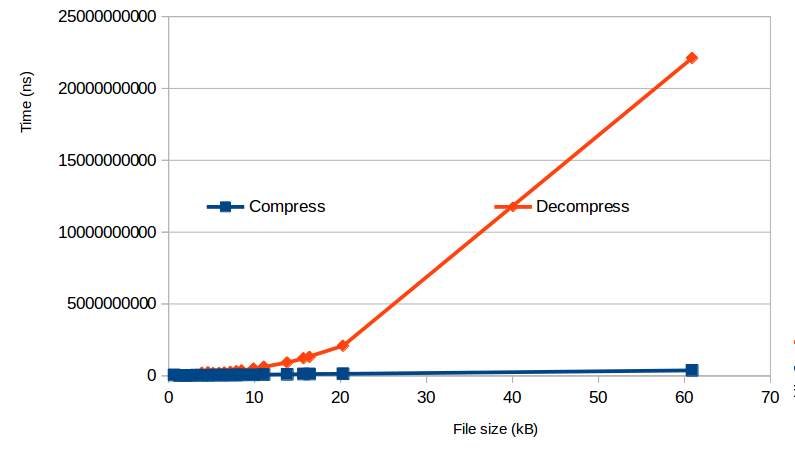
\includegraphics[scale=0.4]{graph.png}
\end{figure}

La complexité temporelle de notre décompression est en $\Theta(n^2)$ où n représente le nombre de caractères dans le fichier décompresser, ce qui correspond approximativement à la courbe rouge se trouvant sur la figure. Néanmoins, la complexité que nous avions calculée pour la compression O(n*m), où n et m représentent le nombre de lignes et le nombre de caractères de la plus longue ligne présente dans le fichier à compresser), ce qui ne correspond pas à la courbe bleue qui semble évoluer d'avance linéairement. 
\subsubsection*{Question 10}
Lors de la compression, les retours à la ligne ne sont pas pris en compte. Ainsi, lorsque le texte est décompressé, celui-ci se retrouve sur une seule ligne. A part cet inconvénient, la compression et la décompression sont sans perte. 

Pour tester cela nous avons utilisé un texte comportant divers types de caractères. 

\end{document}
